\documentclass[kulak]{kulakarticle} % options: kulak (default) or kul

\usepackage[dutch]{babel}
\usepackage{pdfpages}
\usepackage{graphicx}
\usepackage{mathtools}
\usepackage{nccmath}
\usepackage{cprotect}


\title{Smart Fire Extinguisher - Tussentijds Verslag}
\author{TEAM 6: Anna-Laura, Emile, Jérôme, Jesse}
\date{Academiejaar 2022 -- 2023}
\address{
	\textbf{Groep Wetenschap \& Technologie Kulak} \\
	Ingenieurswetenschappen \\
	P\&0 2}

\begin{document}

\maketitle

\section*{Inleiding}

Bij de brandbestrijding in grote warenhuizen worden momenteel sprinklers gebruikt. Deze zijn vastgemaakt aan het plafond van het gebouw en zijn aan de waterleiding aangesloten om bij brand water te doen neerdalen en de brand te blussen. Ze werken heel efficienten, maar hebben wel grote nadelen. De voornaamste zijn de kost van de aanleg en het onderhoud van alle leidingen die de sprinklers van water voorzien. Bovendien kan er bij schade aan de waterleidingen veel water verloren gaan en waterschade optreden. \\

Daarom zijn wij op zoek gegaan naar een efficientere manier om branden te blussen. Een \textbf{Smart Fire Extinguisher}, die zelf de branden kan detecteren, localiseren en gericht kan blussen. Zo zou 1 apparaat (met dus maar 1 aansluiting op de waterleiding of een eigen waterreservoir) een groot oppervlakte brandveilig kunnen maken. Dit zou het veel goedkoper maken voor de eigenaar die geen eindeloos lange waterleidingen moet aanleggen en onderhouden. De totale kost voor grote warenhuizen zou dus veel lager liggen en de kans op waterschade bij het springen van waterleidingen is veel kleiner.


\section{Ontwerp}
\subsection{Klantenvereisten}

De klant verwacht een apparaat dat zelfstandig branden kan detecteren en deze kan blussen. Hiervoor moet het de exacte locatie van de brand kunnen vaststellen en de arm in de juiste richting richten. Het apparaat moet water vanuit een jerrycan in de richting van de brand spuiten en zelf stoppen wanneer de brand geblust is. 

Alles moet automatisch werken, maar er moet ook een manuele override zijn waarbij het apparaat volledig manueel kan worden bestuurd en worden uitgeschakeld. Al dit moet gebeuren in communicatie met een PC. 

\subsection{Ontwerpspecificaties}
\begin{itemize}
	\item Branden detecteren en blussen in een rechthoek van 7m x 6m op 3m afstand 
	\item Maximale uitwijking horizontaal: 90°  
	\item Maximale uitwijking verticaal: 90°
	\item Minimale spuitdruk: … 
	\item Hoeveelheid water per blussing: (wordt nog bekend gemaakt, foutenmarge nog inrekenen) 
	\item Hoeveelheid beschikbaar water: 10L 
	\item Elektronica afgeschermd van water 
	\item Massa robot: max. 20 kg
\end{itemize}

\subsection{Ontwerp}
We opteren voor een \textbf{stationair brandblusplatform} dat gebruik maakt van een draaiend platform en een arm om het water in de juiste richting en onder de juiste hoek weg te spuiten. Water uit een waterreservoir zal dan met behulp van een pomp op de gewenste plaats terecht komen. De plaats zal zijn vastgesteld door een camera. Deze detecteert de brand en aan de hand van de beelden zal er berekend worden waar en hoe ver de brand zich bevindt ten opzichte van het brandblusplatform. Daarna zullen nog een hoop berekeningen de hoek van de twee armen bepalen. \\

Voor \textbf{de detectie} van de brand maken we gebruik van een webcam (USB Webcam 1080P), in Python wordt een programma geschreven op een laptop die aan branddetectie en -localisatie doet. De camera is vastgemaakt op het roterend platform. \\

\textbf{Het richten} van het draaiend platform en de arm gebeurt met behulp van twee motoren (Micro Metal Gear Motor 100:1 HP), deze zullen dankzij een motor driver met de gewenste snelheid en in de juiste richting draaien. Volgens de berekeningen gedaan door een laptop en webcam zullen de armen juist geposisioneerd worden. \\

Wanneer de arm correct gericht is, is de laatste stap \textbf{het blussen} van de brand. Hiervoor zal de pomp (Membraanpomp 12V 4.8 bar) water uit het waterreservoir (jerrycan 10L) door een slang (met diameter 10mm) pompen, om zo weggespoten te worden richting het doelwit. De benodigde afstand halen om het volledige bestrijkingsgebied te kunnen bestrijken is mogelijk door het aanpassen van het mondstuk.


\section{Berekeningen en code}
\subsection{Hoek van de waterstraal}
\subsubsection{Berekening}
De afstand zoals te zien in afbeelding \ref{schematische voorstelling} tussen het brandblusapparaat en de cilinder is \(x\) waarbij \(x\) maximaal gelijk kan zijn aan \(10,45 m\). Om deze afstand te halen berekenen we de hoek waaronder het water moet worden weggespoten. De hoogte van het platform is hier \(h_1\) en de hoogte van de arm is \(h_2 = lsin(\theta)\) met \(l\) de lengte van de arm. \(y\) is de hoogte van de cilinder die moet worden opgevuld. Dan krijgen we:
\begin{equation}
	\begin{cases}
		x  = cos(\theta) v t \\
		y = h_1 + h_2 + sin(\theta) v t + \frac{-1}{2} g t^2
	\end{cases}
\end{equation}
Bij het gebruik van de brandblusser zullen we met behulp van de camera \(x\) al kennen, dankzij de waterflowsensor zullen we \(v\) ook accuraat kennen, \(h_1\) staat vast en \(h_2\) hangt af van de hoek \(\theta\). Uit de twee vergelijkingen kunnen we \(\theta\) en \(t\) halen en zal het doelwit gevuld geraken.

\subsubsection{Code}
De functie \verb*|hoekV(waterDebiet,afstandBeker)| (zie figuur \ref{flowchart_water}) berekent de hoek \(\theta\)  die nodig is tussen het platform en de arm. Deze functie heeft daarvoor het waterdebiet, in \(l/min\), nodig en de verticale afstand, in \(m\), tot het doelwit. Het waterdebiet wordt meegegeven door de waterflowsensor en de afstand door de webcam. Er worden ook niet-variabele parameters gebruikt die op voorhand zijn vastgelegd, zoals de straal van het spuitgat, de hoogte van het platform, de lengte van de arm, de hoogte van het doelwit en de afstand tussen het beginpunt van de arm en de camera. 

In deze functie wordt dan de snelheid van het water berekend en dat wordt in een stelsel gebruikt met twee vergelijkingen. Dit stelsel wordt, met gebruik van de scipy-package, opgelost naar de hoek \(\theta\) en de tijd \(t\).
\begin{equation}
	\begin{cases}
		afstandBeker  = cos(\theta )*lengteArm - afstandCamera + cos(\theta )*snelheid*t \\ 
		hoogteBeker  =  hoogtePlatform + sin(\theta )*lengteArm + sin(\theta )*snelheid*t - 1/2*9.81*t^2
	\end{cases}\,.
\end{equation}
De hoek \(\theta\) wordt omgezet van radialen naar graden en is dan de output van deze functie en kan dan gebruikt worden voor één van de motoren.

\begin{figure} [h!]
	\centering
	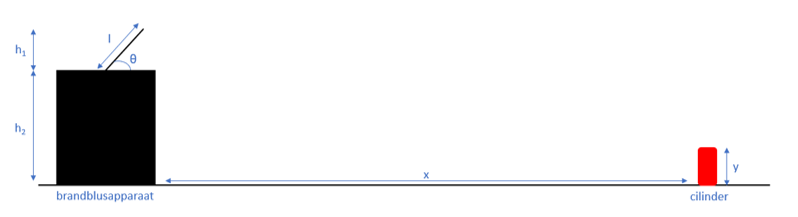
\includegraphics[width = 1 \textwidth]{schematische voorstelling water LATEX}
	\caption{Schematische voorstelling van de opstelling}
	\label{schematische voorstelling}
\end{figure}

\begin{figure} [h!]
	\centering
	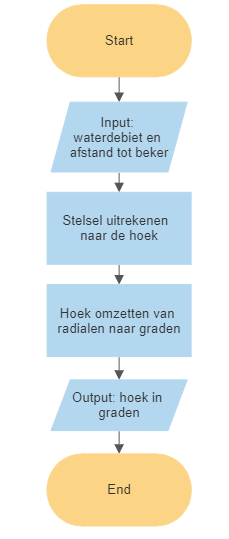
\includegraphics[width = .2 \textwidth]{flowchart_hoekV}
\cprotect\caption{Flowchart van de functie \verb*|hoekV(waterDebiet,afstandBeker)|}
	\label{flowchart_water}
\end{figure}




\subsection{Stoppen met water spuiten}
\subsubsection{Berekening}
Wanneer de hoeveelheid water nodig om een brand te blussen bekend wordt gemaakt en we een foutenmarge uit een handvol experimenten hebben berekend zullen we de hoeveelheid aan onze code kunnen toevoegen. De foutenmarge zal een gemiddelde zijn van water die naast het doelwit terecht komt. We zullen gebruik maken van de aangekochte waterflowsensor om de exacte hoeveelheid uitgespoten water te bekomen. 




\subsubsection{Code}
\begin{figure} [!h]
	\centering
	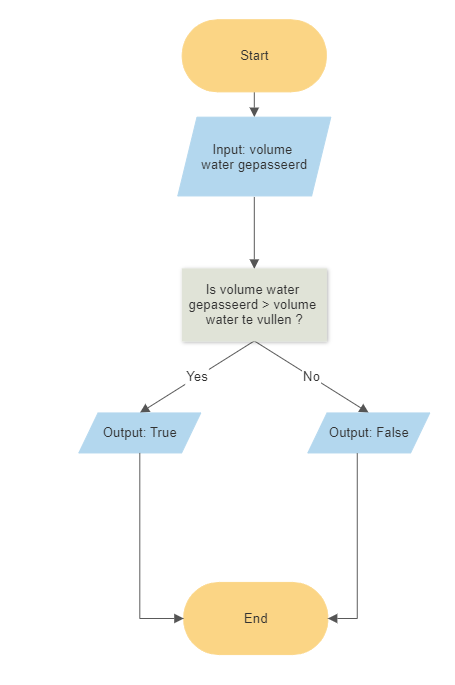
\includegraphics[width = .4 \textwidth]{flowchart_stoppenPompen}
\cprotect\caption{Flowchart van de functie \verb|stoppenPompen()|}
\end{figure}





\subsection{Camera}
\subsubsection{Berekening}
Omdat het gezichtsveld van de camera niet het volledige bestrijkingsgebied omvat (zie figuur \ref{bestrijkingsgebied}), hebben we besloten de camera te laten meedraaien met het draaiende platform. 
\begin{figure} [h!]
	\centering
	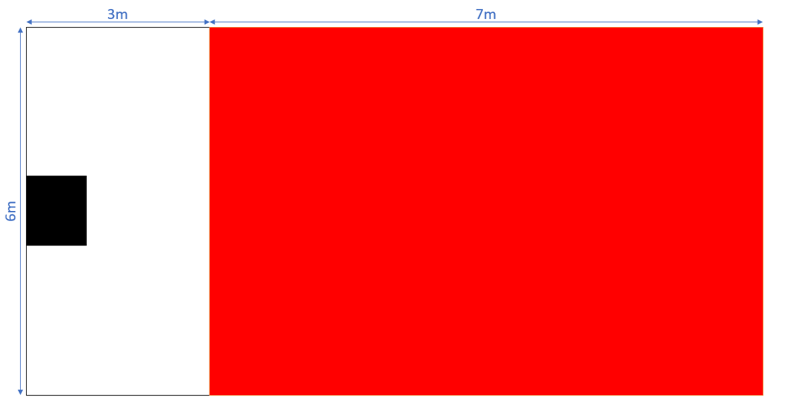
\includegraphics[width = .75 \textwidth]{schematische voorstelling bestrijkingsgebied LATEX}
	\caption{Schematische voorstelling van het bestrijkingsgebied}
	\label{bestrijkingsgebied}
\end{figure}

\subsubsection{Code}

\begin{figure}
	\centering
	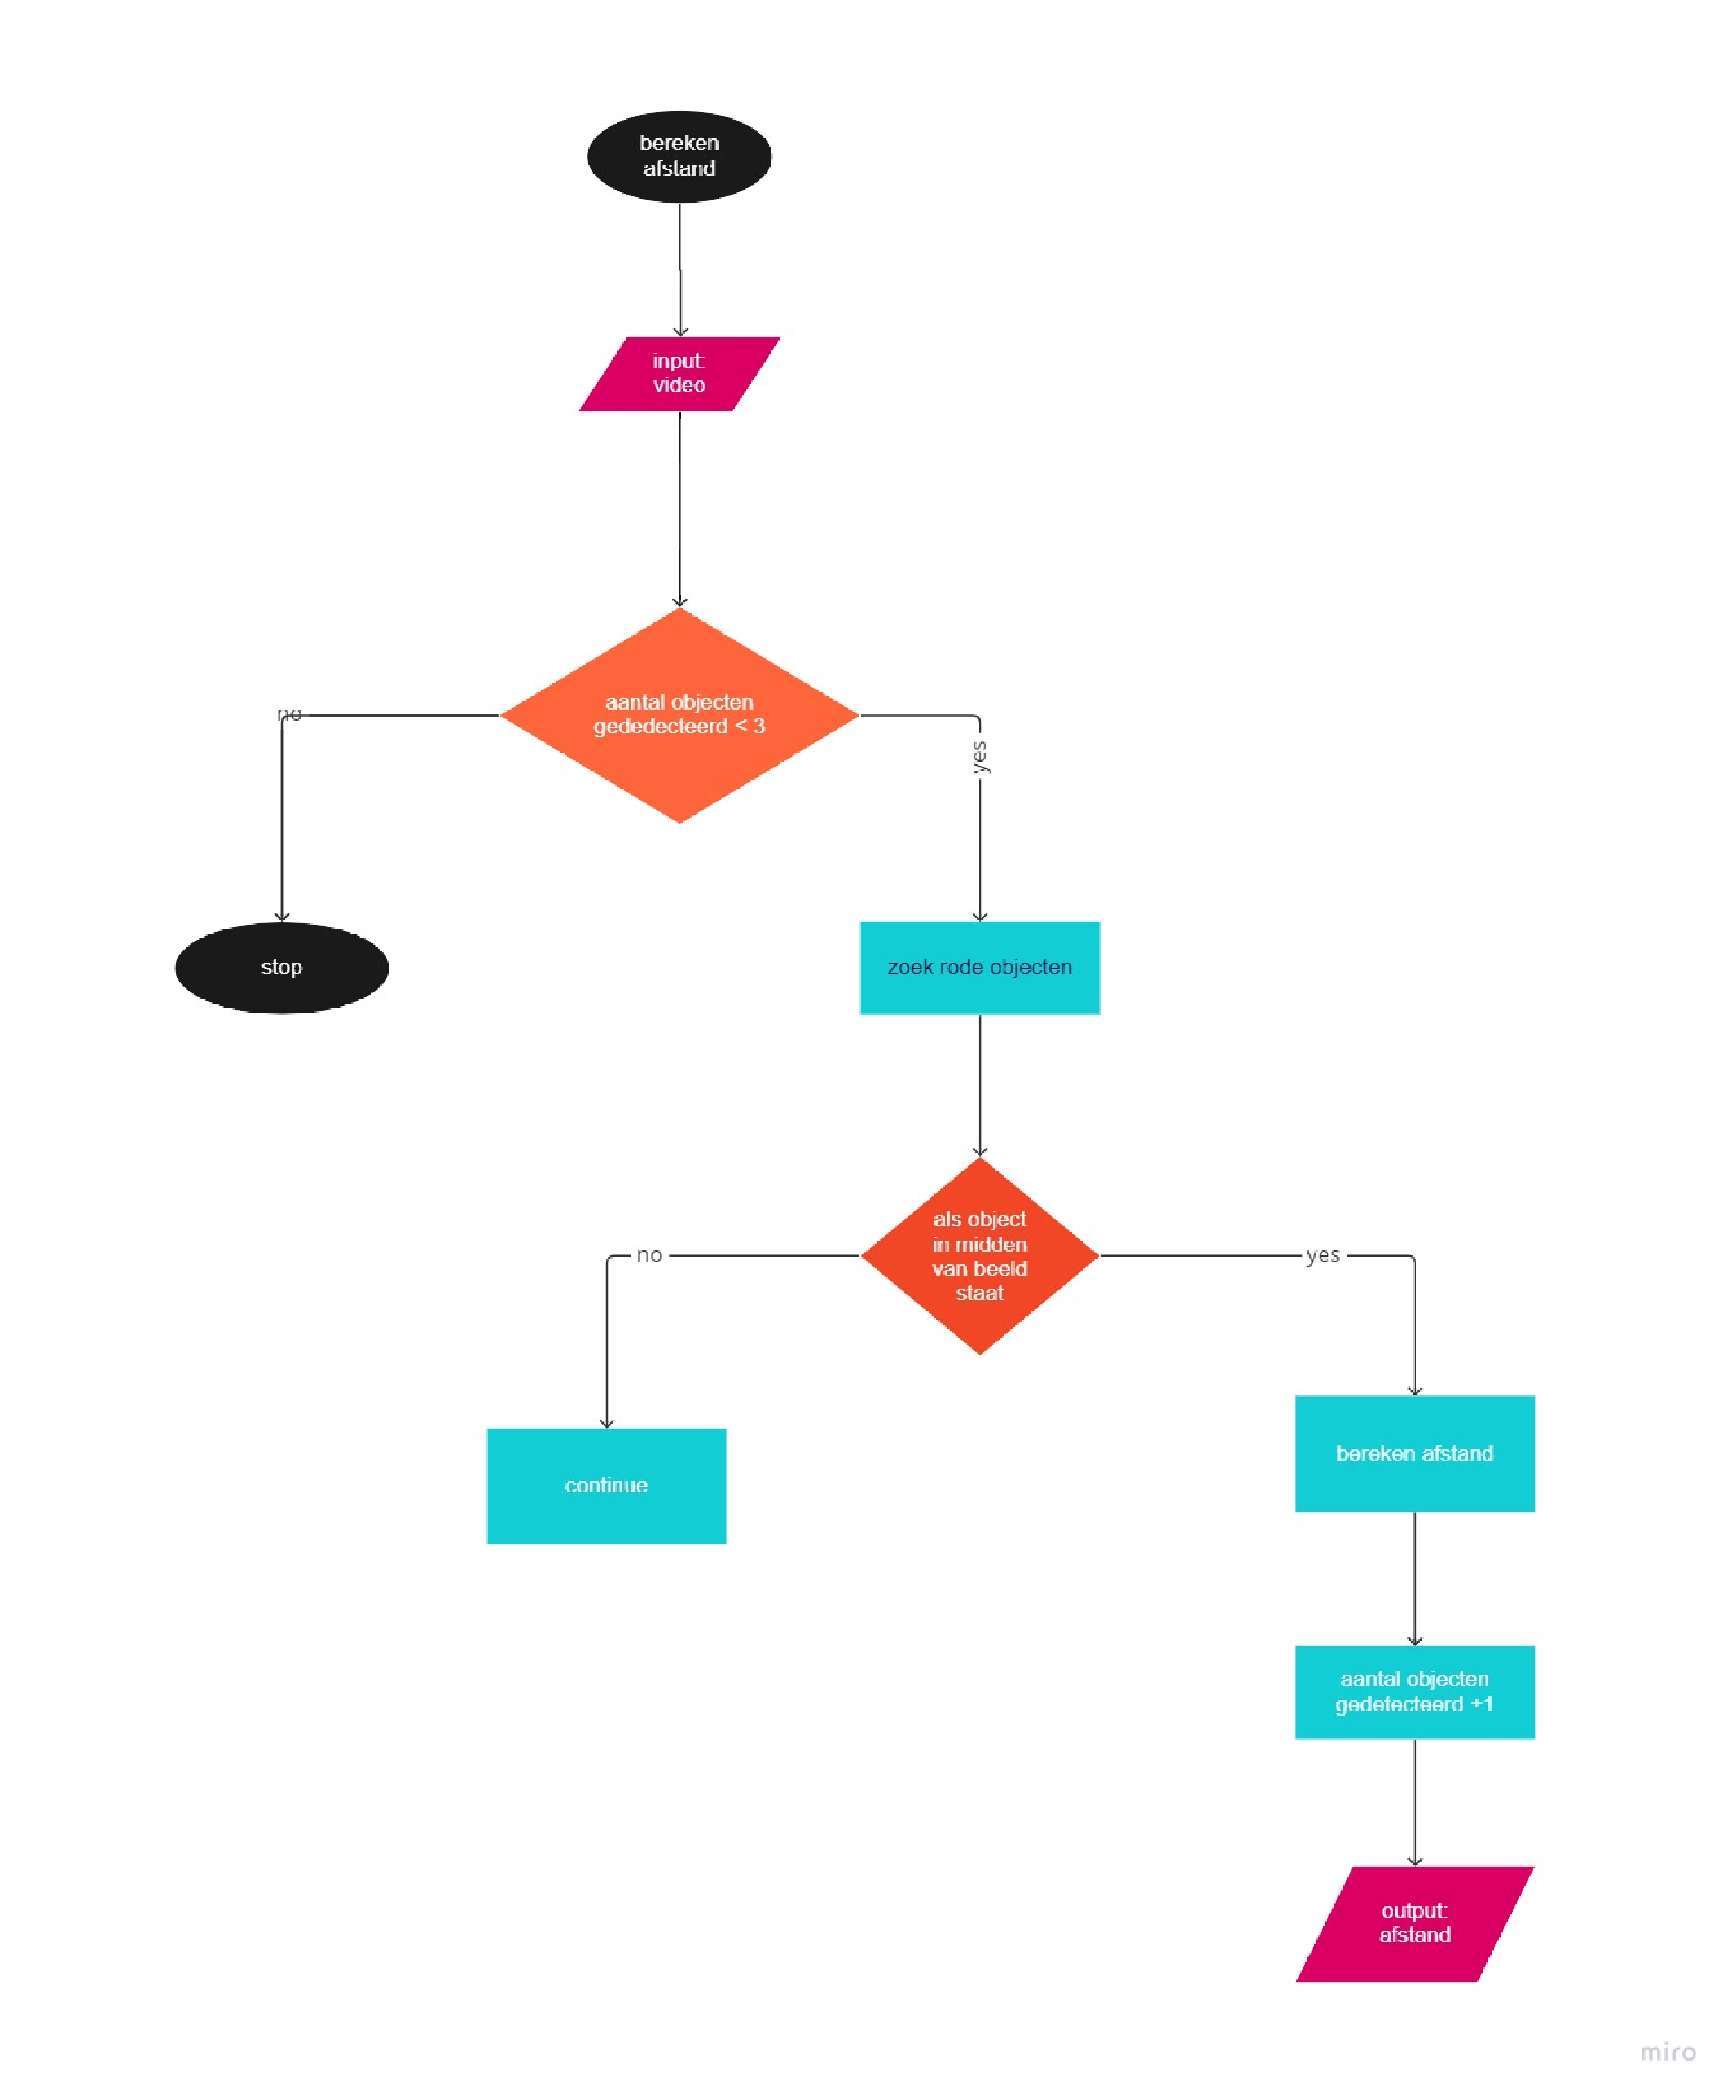
\includegraphics[width = 0.8 \textwidth]{flowchart afstand berekenen.pdf}
	\caption{Flowchart van de functie ...}
\end{figure}
 



\section{Planning}
Op de pagina hieronder is onze taakstructuur te vinden. De eerste taak, het verkennen van de opdracht, is al voltooid. Ons CAD model is bijna af en we zijn al begonnen met het coderen van de microcontroller en PC alsook met de bouw van het geraamte van ons apparaat. 
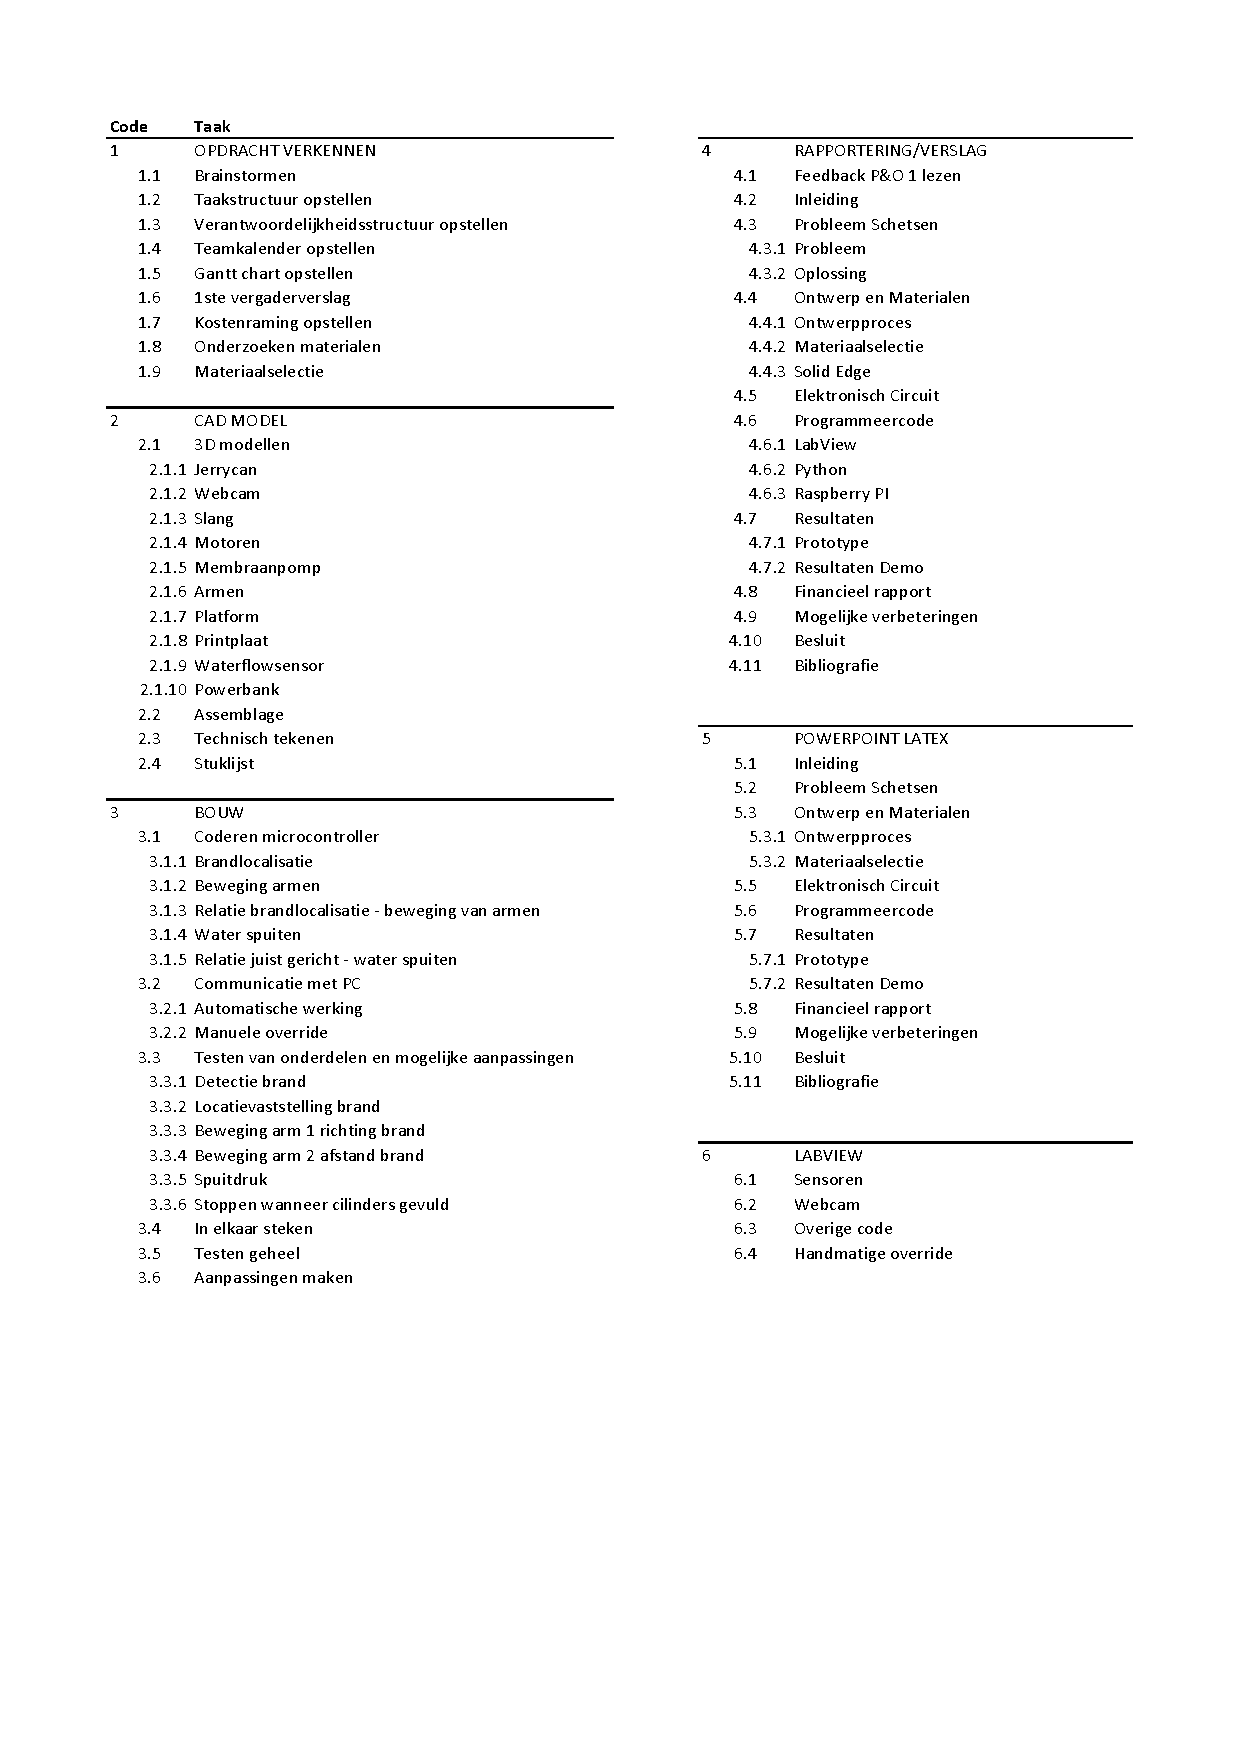
\includepdf{taakstructuur_LATEX_2.pdf}


\end{document}
